\titledquestion{Liveness analysis}
\droptotalpoints

Consider the following intermediate code:

\begin{center}
\begin{minipage}{5cm}
\fvset{frame=lines}
\fvset{framesep=8pt}
\begin{Verbatim}
     c := r3
     a := r1
     b := r2
     d := 0 
     e := a      
l1:  d := d + b
     e := e - 1
     if e > 0 goto l1
     r1 := d
     r3 := c
     return     
\end{Verbatim}
\end{minipage}
 \end{center}

\begin{parts}
\part[2]
Construct the control graph.
\part[3]
Calculate successor nodes, defined variables, and used variables for each node
in the control graph.
\part[15]
Assume \verb+r1+ and \verb+r3+ to be live-out on the return instruction.
Calculate live-ins and live-outs for each node in the control graph.
Present your results in a table.
\end{parts}

\begin{solution}
\\\vtop{\vskip-8pt
  \hbox{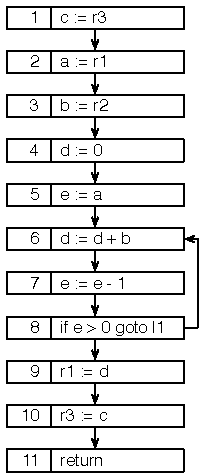
\includegraphics[scale=.85]{questions/register-allocation/controlflow-appel-11-3-1}}
  }
\begin{tabular}[t]{r|l>{\ttfamily}l>{\ttfamily}l|>{\ttfamily}l>{\ttfamily}l|>{\ttfamily}l>{\ttfamily}l}
node & succ & \textnormal{def} & \textnormal{use} & \textnormal{out} &
\textnormal{in} & \textnormal{out} & \textnormal{in} \\
\hline
11 &        &    &     & r1 r3   & r1 r3    & r1 r3   & r1 r3   \\
10 & 11     & r3 & c   & r1 r3   & r1 c     & r1 r3   & r1 c    \\
 9 & 10     & r1 & d   & r1 c    & c d      & r1 c    & c d     \\
 8 &  6, 9  &    & e   & c d     & c d e    & b c d e & b c d e \\
 7 &  8     & e  & e   & c d e   & c d e    & b c d e & b c d e \\
 6 &  7     & d  & b d & c d e   & b c d e  & b c d e & b c d e \\
 5 &  6     & e  & a   & b c d e & a b c d  & b c d e & a b c d \\
 4 &  5     & d  &     & a b c d & a b c    & a b c d & a b c   \\
 3 &  4     & b  & r2  & a b c   & r2 a c   & a b c   & r2 a c  \\
 2 &  3     & a  & r1  & r2 a c  & r1 r2 c  & r2 a c  & r1 r2 c \\
 1 &  2     & c  & r3  & r1 r2 c & r1 r2 r3 & r1 r2 c & r1 r2 r3
\end{tabular}
\end{solution}
